\chapter{Selective Capture and Replay for Eiffel}
In the following we will describe how we implemented selective capture and replay for Eiffel with an emphasis on the differences to the original Java implementation. The chapter ends with a section that describes how to build our implementation from source and run an Eiffel example of selective capture and replay.

\eiffellisting
\section{Differences to Existing Implementation}
Selective capture and replay as described by Joshi and Orso \cite{orso05may} can not be directly applied to Eiffel. The core elements of the technique can be applied to Eiffel, but it is necessary to adjust some parts. In this section the changes to the original implementation and reasons for these changes will be discussed.

\subsection{Language Aspects}
Even though Java and Eiffel are both object oriented languages, there are differences between these two languages, syntax left aside. Eiffel offers a wider set of language constructs, many times trying to solve problems inherently object oriented, whereas Java reused solutions from its ancestors, mainly C++. One example for this difference are be the Eiffel basic types, which can be treated as objects with methods versus the Java basic types, which are no objects. This section focuses on the differences between Java and Eiffel that influenced our implementation of selective capture and replay.

\subsubsection{Terminology} % diesen Titel weglassen?
Eiffel has a nomenclature that differs from other programming languages. Here the Eiffel terminology is described according to Meyer's Book \cite{oosc2} and compared to the one from Java.
\begin{center}
\begin{tabular}[]{|l|l|} \hline
 \textbf{Eiffel}&\textbf{Java} \\ \hline
 Attribute&Field \\ \hline
 Query&Field or Method that has a return value \\ \hline
 Routine&Method \\ \hline
 Procedure&Method that has no return value \\ \hline
 Function&Method that has a return value \\ \hline
 Feature&Method or Attribute \\ \hline
 ANY&Object (ancestor of all classes) \\ \hline
\end{tabular} 
\end{center}

\subsubsection{Multiple Inheritance}
Eiffel is designed to support multiple inheritance, whereas in Java, only single inheritance is allowed. The original implementation assumes, that all subclasses of a class \emph{c} are in the observed set iff \emph{c} is also in the observed set. This makes it possible to statically decide whether an observed or an unobserved feature is accessed.

If this assumption is translated to multiple inheritance, it would not be possible to have a class \emph{C} that inherits both from an observed class \emph{A} and an unobserved class \emph{B} (\figref{fig:obs_unobs_multiple_inheritance}).
\begin{figure}[ht]
  \centering
  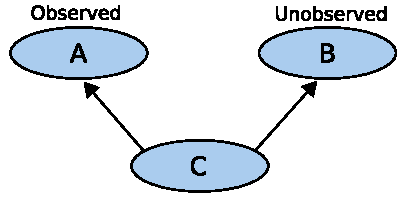
\includegraphics[width=0.5\textwidth]{illustrations/obs_unobs_multiple_inheritance}
  \caption{Conflict Between Observed and Unobserved Set Due to Multiple Inheritance}
  \label{fig:obs_unobs_multiple_inheritance}
%\includegraphics{illustrations/capture_and_replay_generic_structure}
\end{figure}

Multiple inheritance is extensively used in Eiffel, thus this assumption is too restrictive, because it leads to big clusters of classes that either all must be observed or all unobserved.

Although Java does not allow multiple inheritance, it supports multiple interface inheritance. Joshi and Orso \cite{orso05may} mention that they need to dynamically determine if the target of an event is observed or unobserved in certain cases. We assume that multiple interface inheritance with a class that both implements an observed and unobserved interface  is at least one of these cases. SCARPE uses the \identifier{instanceof} operator to determine if an object is an instance of an observed class. For example if in our application \class{ATM\_UI\_TEXTUAL} is observed and the class \class{ATM\_UI\_GRAPHICAL} is unobserved, variables of type \class{ATM\_UI} can reference an instance of an observed \emph{or} an unobserved class. In that case, it is possible determine with the following Java code whether the actual object is an instance of an observed class:
\javalisting
\begin{lstlisting}
 if(ui instanceof ATM_UI_TEXTUAL){
    /*Instrumentation for instance of observed class*/
 }else{
   /*Instrumentation for instance of unobserved class*/
 }
\end{lstlisting}
\eiffellisting

We will present a solution that always determines dynamically, if an object is an instance of an observed class (\emph{observed object}) or an instance of an unobserved class (\emph{unobserved object}) and a proposal how to solve this problem without reflection.

\subsubsection{Read Only Attributes}
Eiffel strictly follows the \emph{uniform access principle} \cite{oosc2}. The principle states that it should not be visible to the clients whether features are implemented through storage or computation. This ensures that the implementation of a feature can be changed from attribute to function or vice versa. One of the consequences of this principle is that clients of a class cannot write to attributes, as these attributes could be implemented as a function as well.

In Java, this principle is not ensured because clients of a class can write to their fields. For our implementation of selective capture and replay, this limits the events related to field accesses to OUTREAD. Both OUTWRITE and INWRITE can not happen, because write access to fields is restricted to their class, thus there can be no write accesses to fields from observed to unobserved classes or reverse.

\subsection{Target Application}
As a first application that could use selective capture and replay in Eiffel, Cdd, a tool for contract driven development \cite{cdd07} was chosen. Cdd allows programmers to extract test cases from failing program runs. The contracts that are present in the code are used as test oracles. Cdd is not always able to generate such a test case, due to different reasons:

\begin{description}
\item [Prestate extraction:] The state before calling the failing feature (which is needed to generate a test case) is extracted using the state at the time of failure. Because not all instructions between feature call and failure can be undone, the extraction of the prestate is not always possible.
\item [Non-determinism:] If the failing feature reads values from sources that don't always return the same values (e.g. user input), it's not generally possible to run the test cases with the same result as in the failing run.
\item [External state:] When the feature relies on state that is not stored in Eiffel objects, for example in C structs, Cdd is not able to gather this state for the test.
\end{description}

All these limitations can be resolved using selective capture and replay:
\begin{description}
\item [Prestate extraction:] By setting a breakpoint at the beginning of the failing feature, it is possible to extract the prestate during the replay of the application.
\item [Non-determinism:] When adding all non-deterministic classes to the unobserved set, it can be ensured that the replay of the run is deterministic.
\item [External State:] All classes that wrap external state can be added to the unobserved set. Thus interactions with these classes can be replayed without having to store the external state.
\end{description}

Prestate extraction using selective capture and replay requires an immediate rerun of the application under test. Because complete recompiles in Eiffel last for tens of minutes up to hours, we can not afford to instrument the application again before replaying it. Thus it is necessary to design the code instrumentation to be applicable for both capture \emph{and} replay phase. We pushed this approach even further to allow the user to disable the whole instrumentation. This allows execution with minimal overhead if capture and replay is not needed, without recompiling the application.

\section{Code Instrumentation}
One of the key elements of selective capture and replay is code instrumentation, which is necessary to detect events that are relevant for the replay phase. In the following we will describe how application code is instrumented in order to detect events and how this instrumentation is inserted at compile time.

\subsection{Outline}
Due to differences between Eiffel and Java and a different use case, there are two main changes between the original implementation and our approach:

\begin{enumerate}
 \item It is necessary to determine dynamically whether an object is observed or not.
\item It must be possible to switch between capture and replay phase without re-instrumenting the code.
\end{enumerate}

The first requirement can be met by adding an additional query to every class so that it is possible to find out whether an object is an instance of an observed or an unobserved class. We ensure that every class has this query by adding it to \class{ANY}. In Section \ref{lbl:is_observed} we will discuss how this query can be implemented efficiently.

In order to be able to switch between capture and replay mode, the class \class{PROGRAM\hspace{0pt}\_FLOW\hspace{0pt}\_SINK} was introduced. Program flow events are put into the \class{PROGRAM\hspace{0pt}\_FLOW\_SINK}. It is both the ancestor class of \class{RECORDER}, the class that contains the management code for recording events and \class{PLAYER}, the class that provides the scaffolding for replaying events. The standard instance of a \class{PROGRAM\hspace{0pt}\_FLOW\_SINK} is globally accessible. It is dynamically bound to an instance of \class{RECORDER} during capture phase and \class{PLAYER} during replay phase.

To create placeholder objects from unobserved classes, their original routine bodies are disabled during replay phase. When replaying, the routines only execute instrumentation code that invokes the scaffolding and takes care of the return value if necessary.

\subsection{Routines}
Whereas the original implementation captures routine calls by instrumenting the call site (in the client), we decided to instrument the calee (the supplier). This simplifies code instrumentation, because there is no need to make changes inside existing routine bodies; it is sufficient to add some code at the beginning and the end of the routine bodies. %TODO Gibt es noch ein besseres Motiv?

The routine instrumentation can be divided into three parts (\figref{fig:routine_instrumentation_structure}): right at the beginning of the routine, code to detect call events is inserted. The original routine body is made conditional so that it is not executed for unobserved routines during the replay phase. Finally, code to detect callret events is inserted at the end of the routine.
\begin{figure}[ht]
  \centering
  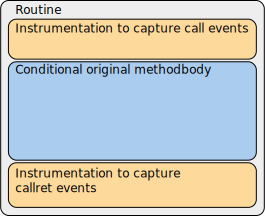
\includegraphics[width=0.5\textwidth]{illustrations/routine_instrumentation_structure}
  \caption{The Three Sections of Routine Instrumentations}
  \label{fig:routine_instrumentation_structure}
\end{figure}

To explain instrumentation in more detail, we describe each of these three parts using the query \feature{account\_exists} of the class \class{ATM} (\listref{lst:account_exists_original}).

\begin{lstlisting}[caption=Original Code of Query \feature{account\_exists} ,label=lst:account_exists_original]
account_exists (account_name:STRING): BOOLEAN
		-- Is there an account with name 'account_name'?
	require
			account_name_not_void: account_name /= Void
	do
		Result := (the_bank.account_for_name (account_name) /= Void)
	end
\end{lstlisting}

\subsubsection{Capturing Call Events}
To capture call events, instrumented code, which is only executed when capture and replay is enabled, is inserted at the beginning of every routine. The code first detects whether the routine was called across the boundaries. If that is the case, it puts the associated event into the program flow (\listref{lst:invocation_instrumentation}).
\begin{lstlisting}[caption=Instrumentation Code to Detect Call Events,label=lst:invocation_instrumentation]
if program_flow_sink.is_capture_replay_enabled then
	program_flow_sink.enter
	if program_flow_sink.observed_stack_item /= is_observed then
		program_flow_sink.put_to_observed_stack (is_observed)
		program_flow_sink.put_feature_invocation ("account_exists", Current, [account_name])
	else
		program_flow_sink.put_to_observed_stack (is_observed)
	end
	program_flow_sink.leave
end
\end{lstlisting}
Note that all the inserted code is part of the selective capture and replay management code, which does not belong to the code of the original application, thus these instructions must not trigger further events for the event log. For example the creation of the manifest string ``account\_exists'' should not create other call events on class \class{STRING}. To make sure, that this will not happen, the commands \feature{enter} to disable capture and replay and \feature{leave} to re-enable capture and replay were introduced.

To detect boundary crossing calls, the management code keeps an own stack that indicates whether the target objects of the calls on the call stack are observed or not. This stack is managed in parallel to the call stack; in the invocation instrumentation code, the result of the query \feature{is\_observed} is put onto the stack and in the exit instrumentation code, this value is removed again. Using this stack, it is possible to find out, whether the caller object is observed or not.


\subsubsection{Conditional Routine Body Execution}
To be able to switch between the original and the placeholder routine body, the original routine body of unobserved routines is only executed during capture phase (\listref{lst:methodbody_instrumentation}). Placeholder routines are only needed for unobserved routines, thus the original body is always executed for observed routines . The query \feature{is\_replay\_phase} indicates if the program is running in replay mode; it always returns false, when capture and replay is disabled, therefore the management code will always use the original routine body.

\begin{lstlisting}[caption=Conditional Methodbody,label=lst:methodbody_instrumentation]
if (not program_flow_sink.is_replay_phase) or is_observed then
	Result := (the_bank.account_for_name (account_name) /= Void)
end
\end{lstlisting}


\subsubsection{Capturing Callret Events}
To capture and replay callret events, instrumentation code is inserted at the end of routines. Again, the code only puts an event into the \feature{program\_flow\_sink} if the routine was called across the boundary. For functions, the code also restores the result to \feature{program\_flow\_sink\_.last\_result}, which has only an effect for unobserved functions during replay phase, otherwise the query \feature{last\_result} returns the same value that was put into the \feature{program\_flow\_sink} before. Thus functions can be used as placeholder functions without altering the instrumentation between capture and replay phase.
\begin{lstlisting}[caption=Instrumentation to Capture Callret Events,label=lst:exit_instrumentation]
if program_flow_sink.is_capture_replay_enabled then
	program_flow_sink.enter
	program_flow_sink.remove_from_observed_stack
	if program_flow_sink.observed_stack_item /= is_observed then
		program_flow_sink.put_feature_exit (Result)
		Result ?= program_flow_sink.last_result
	end
	program_flow_sink.leave
end
\end{lstlisting}


\subsubsection{Complete Routine Instrumentation}
\listref{lst:account_exists_instrumented} shows the routine after combining all three parts of the instrumentation.
\begin{lstlisting}[caption=Routine \feature{account\_exists} After Instrumentation,label=lst:account_exists_instrumented]
account_exists (account_name: STRING_8): BOOLEAN
		-- Is there an account with name 'account_name'?
	require
		account_name_not_void: account_name /= Void
	do
		if program_flow_sink.is_capture_replay_enabled then
			program_flow_sink.enter
			if program_flow_sink.observed_stack_item /= is_observed then
				program_flow_sink.put_to_observed_stack (is_observed)
				program_flow_sink.put_feature_invocation ("account_exists", Current, [account_name])
			else
				program_flow_sink.put_to_observed_stack (is_observed)
			end
			program_flow_sink.leave
		end
		if (not program_flow_sink.is_replay_phase) or is_observed then
			Result := (the_bank.account_for_name (account_name) /= Void)
		end
		if program_flow_sink.is_capture_replay_enabled then
			program_flow_sink.enter
			program_flow_sink.remove_from_observed_stack
			if program_flow_sink.observed_stack_item /= is_observed then
				program_flow_sink.put_feature_exit (Result)
				Result ?= program_flow_sink.last_result
			end
			program_flow_sink.leave
		end
	end
\end{lstlisting}


\subsection{Attribute Accesses}
Automated code instrumentation for attribute accesses could not be developed as part of this thesis, because the part of the Eiffel compiler code, that was intended to be used for instrumentation, turned out to be unsuitable for the task. Emmanuel Stapf of Eiffel Software inc. advised us to use the mechanism that generates wrapper code for attribute accesses to support expanded generic derivation reattachment (related to autoboxing). Unfortunately the compiler could not apply the mechanism to all attribute accesses and it was not possible to make the necessary changes in the compiler due to a lack of time.

Here is a sketch how the instrumentation code for an access to \inlineeiffel{atm.ui} could look like:
\begin{lstlisting}[caption=Instrumentation of an Attribute Access]
 if program_flow_sink.is_capture_replay_enabled  and then is_observed and then (not atm.is_observed) then
	program_flow_sink.enter
	program_flow_sink.put_attribute_access("ui",atm, atm.ui)
	program_flow_sink.leave
 end
 ui := atm.ui
\end{lstlisting}
Again, the instrumentation code can be used for both capture and replay phase. The condition makes sure, that only OUTREAD events are captured and replayed. During capture phase, the \class{RECORDER} logs the corresponding OUTREAD event and during replay phase, the \class{PLAYER} ensures that the value of the attribute read in the next statement corresponds to the value that was read during capture phase, by setting the attribute to the value from the log.

The whole instrumentation needs to be put into a function that is accessed instead of the attribute, because the attribute can be accessed as part of a more complex expression:
\begin{lstlisting}
 a := other.function + other.attribute
\end{lstlisting}
It does not suffice to execute the instrumentation for the access to \inlineeiffel{other.attribute} one instruction before the evaluation of the expression, because \inlineeiffel{other.function} could have a side effect that changes \inlineeiffel{other.attribute}; although this violates the \emph{Command-Query Separation Principle} \cite{oosc2}, it can not be forbidden.


\subsection{Attribute Manipulation from C Level}
One assumption of the original selective capture and replay implementation is that native code never manipulates observed fields. Eiffel allows integration of C code into classes, using the \identifier{external} keyword. In order to write to fields of Eiffel objects, the C code needs the address of that object, which is achieved by using the \identifier{\$} - operator.

To find out the classes whose attributes are written from native code, we searched for the \identifier{\$} operator in the Eiffel base library. Only writes to \class{\{STRING\}}\hspace{0pt}.\feature{area} of type \class{SPECIAL [CHARACTER]} were identified to cause problems. Other than that, there were some write accesses to attributes of the class containing the C code, which is unproblematic because these accesses never cross the boundaries.
Restricting the class \class{STRING} to be in the unobserved set was not an option, because it would imply serious performance penalties to applications that heavily use strings (e.g. a parser). To address this issue in a different way, the command \feature{note\_direct\_manipulation} was added to the class \class{SPECIAL}, which needs to be called whenever unobserved C code writes to the fields of \class{SPECIAL}. Due to the lack of other use cases, the command was only designed to support \class{SPECIAL [CHARACTER]}. During the capture phase it writes down the new content of the object and when replaying the corresponding event, that content is restored; thus the objects are in the same state during replay as they were in the capture phase.

Manifest strings are another case where C code writes to strings, because the C code generated by Eiffel Studio allocates and initializes these strings directly. No automated instrumentation for manifest strings was developed, but it could be added by modifying the C macro that is used to generate manifest strings.


\subsection{Compiler Integration}
To insert the instrumentation code automatically, the compiler of Eiffel Studio was modified. The Eiffel Studio compiler has many backends: finalized C code, workbench C code, workbench melted code, Java bytecode and .Net CIL. Workbench code is produced in order to run it from Eiffel Studio; it allows faster compilation times with the drawback that it runs slower than finalized code. The generated code runs on a variety of platforms like Windows, Linux, several Unix operating systems, MacOS X and others \cite{eiffelsoftware}. To support as many backends as possible, one target was to keep the instrumentation code in Eiffel wherever possible, as the backend and platform independence is then guaranteed by the Eiffel compiler. To this end our modifications in the compiler change the abstract syntax tree (AST) before code generation, which is the approach that comes closest to changing the source code of the application directly.

Emmanuel Stapf advised us to make the modifications in the class \class{AST\hspace{0pt}\_FEATURE\hspace{0pt}\_CHECKER\hspace{0pt}\_GENERATOR}, which is used at the stage where the compiler checks the types of the program. Code instrumentation is inserted into the routines before their body is type-checked, in the feature \feature{process\_routine\_as}. Our code generates additional AST nodes and replaces the original AST of the routine body.

A simple mechanism to exclude classes and routines from instrumentation was developed, because some classes like \class{PROGRAM\_FLOW\_SINK} need a special treatment to avoid management code invoking itself through instrumentation code. There are also some features that need to be instrumented in a special way, for example \feature{SPECIAL.note\_direct\_manipulation} that needs to record the content of the instance during capture phase and restore that content during replay phase. To support classes and features that are not to be instrumented, two arrays are initialized with the names of exceptional classes and features. It is clear that at a later stage this needs to be controlled by a configuration file, to avoid recompiling Eiffel Studio, only because these exceptions changed.


\subsection{Alternative Instrumentation}
\label{lbl:single-sided_instrumentation}
One drawback of our implementation is that the whole code is instrumented, whereas in the original implementation of selective capture and replay, only instructions that trigger an event are instrumented. Our implementation can result in a significant performance impairment, therefore we will outline an alternative or extension to our current approach to code instrumentation.

Andreas Leitner proposed to only instrument one of the two parts of the application: either the observed or the unobserved set. Assume in the following, that only the unobserved set is instrumented. With the existing instrumentation of routines, only OUTCALL and OUTCALLRET events would be captured. To capture INCALL and INCALLRET events, it is necessary to instrument all call sites in the unobserved routine bodies. When a routine call is detected, the instrumentation code first determines whether the call crosses the boundary, in which case the management code logs the corresponding event. Before every INCALL, the code sets a global flag that indicates whether code execution is currently in the observed or unobserved set. This will help to identify subsequent calls from observed code to unobserved routines.


\section{Implementation}
In this chapter, we will explain the implementation of the management code. For a quick overview over our implementation, we will first outline the architecture of the solution and then go through the different parts of the management code in the following sections.


\subsection{Outline}
 \figref{fig:implementation_overall_architecture} shows the key classes of the implementation with the \class{PROGRAM\hspace{0pt}\_FLOW\_SINK} as the entrance point to the management code. Program flow events are put into the standard instance of it, which all classes can access through the once function \class{\{ANY\}}\hspace{0pt}.\feature{program\_flow\_sink}. During capture phase, it is set to an instance of \class{RECORDER} and during replay phase, it is set to an instance of \class{PLAYER}.

\begin{figure}[ht]
  \centering
  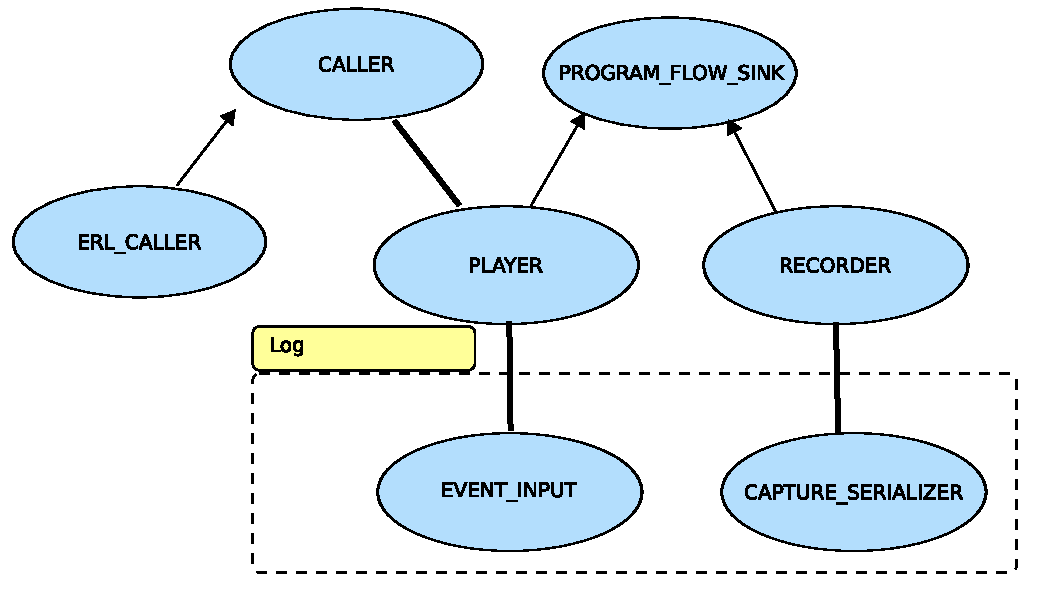
\includegraphics[width=0.8\textwidth]{illustrations/implementation_overall_architecture}
  \caption{Overall Architecture of the Management Code}
  \label{fig:implementation_overall_architecture}
\end{figure}


\subsection{The Event Log}
First it was intended to use XML as the format for the log files because it saves the task of writing a parser and the log file can be verified using XML Schema. For our parser, it was required to parse one event at a time, because the log files can become big when applications are captured over a long time. With the Gobo XML parser, it is not possible to request parsing of a single XML element at a time, there are only the options to use event based parsing or DOM parsing. Using the event based parser was mandatory, because the DOM based parser parses the whole log file and overly allocates memory in order to store all nodes of the DOM tree. The event based mode did not fit, because this required to invoke the replay scaffolding from the parser and not vice versa. One possibility would have been to put the parser into an own thread and block this thread whenever one element is buffered and not yet consumed by the replay scaffolding. Because multi-threading in Eiffel requires a compiler switch which causes alternative, incompatible libraries to be used, this was not an option; it would render the capture/replay mechanism unusable for single threaded applications.
Therefore we decided to implement an own log file grammar (cf. Appendix \ref{sec:log_file_grammar}) with own parser and serializer to be able to incrementally parse the event log on demand.


The classes related to the log were designed to allow addition of other log formats in the future. For example \class{RECORDER} is using the deferred class \class{CAPTURE\_SERIALIZER}, whose descendants can use their own log format (\figref{fig:implementation_serializer}). The deferred class offers a command for each event type to write the corresponding event to the log (e.g. \feature{write\_incall}) and \class{TEXT\_SERIALIZER} implements these commands by writing out the events according to the grammar.

\begin{figure}[ht]
  \centering
  \includegraphics[width=0.5\textwidth]{illustrations/implementation_serializer.png}
  \caption{\class{CAPTURE\_SERIALIZER} and \class{TEXT\_SERIALIZER}}
  \label{fig:implementation_serializer}
\end{figure}

The parser is divided into the class \class{EVENT\_PARSER} that reads from the log and \class{EVENT\hspace{0pt}\_PARSER\_HANDLER} to handle events that were generated by the parser (\figref{fig:implementation_parser}). \class{\{EVENT\_PARSER\}}\hspace{0pt}.\feature{parse\_event} parses the next event from the log and then calls the appropriate handler from \class{EVENT\hspace{0pt}\_PARSER\hspace{0pt}\_HANDLER}, for example \feature{handle\_incall\_event}.  
\class{TEXT\hspace{0pt}\_EVENT\hspace{0pt}\_PARSER} is a \emph{recursive descent parser} \cite{aho86} that parses the line based log file. To support other log formats, it is possible to implement other parsers that inherit from \class{EVENT\_PARSER}.
The player reads events from the class \class{EVENT\_INPUT}, which uses the parser to read the events from the log.

\begin{figure}[ht]
  \centering
  \includegraphics[width=1\textwidth]{illustrations/implementation_parser.png}
  \caption{Architecture of the Event Log Parser}
  \label{fig:implementation_parser}
\end{figure}


\subsection{Object ID}
Selective capture and replay relies on object IDs to be able to capture only partial data. To implement this for Eiffel, an object ID was added to the class \class{ANY} as an additional attribute, which is problematic, because the Eiffel runtime assumes a fixed size for all attributes of \class{ANY}, so it is only allowed to add routines to it. To circumvent this issue, the run-time was  changed to allocate more space for each object. The object ID is stored at the end of the allocated memory to prevent disrupting existing code (\figref{fig:any_object_id}).
\begin{figure}[ht]
  \centering
  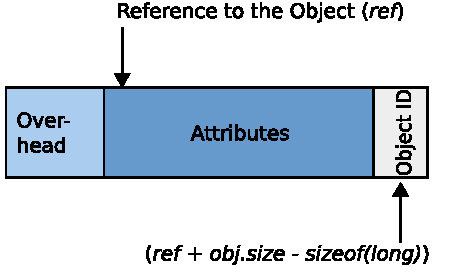
\includegraphics[width=0.4\textwidth]{illustrations/any_object_id}
  \caption{Object ID in the Object Layout of \class{ANY}}
  \label{fig:any_object_id}
\end{figure}

The class \class{SPECIAL}, which is able to store a variable number of elements (used for example for arrays), already makes use of this trick and stores the elements at the beginning and its two attributes \feature{count} and \feature{element\_size} at the end of the allocated area. To avoid a clash with these attributes, the object ID in instances of \class{SPECIAL} is stored between the elements and these two attributes (\figref{fig:special_object_id}). Class \class{TUPLE} also uses a special object layout which renders the approach that was used for \class{ANY} unusable. Due to a lack of time, it was not possible to add support for object IDs to the class \class{TUPLE}.
\begin{figure}[ht]
  \centering
  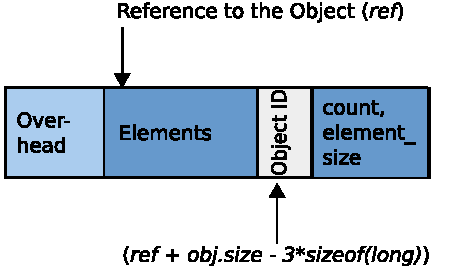
\includegraphics[width=0.4\textwidth]{illustrations/special_object_id}
  \caption{Object ID in the Object Layout of \class{SPECIAL}}
  \label{fig:special_object_id}
\end{figure}

Object IDs are lazily initialized, the first time the function \feature{cr\_object\_id} is called, it retrieves a new object ID from the global counter \feature{cr\_global\_object\_id} and increases that counter. Because the object IDs are not allocated as regular attributes, it is necessary to access them via C code; there are two special C functions in \class{ANY} to read and write the object ID: \feature{c\_object\_id} and \feature{c\_set\_object\_id}.


\subsection{Query to Find out Whether an Object is Observed}
\label{lbl:is_observed}
Because of multiple inheritance, it is not generally possible to determine statically whether an object is observed or not. The original implementation of selective capture and replay uses the Java operator \identifier{instanceof} in special cases to determine the dynamic type of an object, in order to find out whether the object is observed. We decided to add a query to \class{ANY} that facilitates this task. This query can be implemented in different ways: 

\subsubsection{Solution 1: Look up in Hash Set}
The first solution requires a single implementation of the query \feature{is\_observed} that uses a hash set to determine whether an object is observed. By looking up the generating type of the object in a hash set, which contains the names of all classes that are unobserved, the result can be calculated. Querying this implementation of \feature{is\_observed} generates subsequent routine calls, thus the overhead is big, considering the fact that \feature{is\_observed} is invoked three times for each routine call.

\subsubsection{Solution 2: Repeated Redefinition of \feature{is\_observed}}
Another idea is the implementation of a function that is redefined for each class. The function returns always the same value, that is, if the class is observed. The feature can not be a constant attribute, because it is not possible to redefine them, as constant attributes  are resolved at compile time. Implementing the feature as a normal attribute would lead to a unnecessarily high memory consumption, because the value depends only on the class, not the instance.

It is not possible to make a standard implementation for unobserved classes in \class{ANY} and then only redefine it in all observed classes, because there will be conflicting redefinitions, where two ancestors of a class have different redefinitions of the same query \cite{oosc2} (\figref{fig:observed_query_conflicting_redefinitions}). Therefore this feature must be redefined in each class, which must be done automatically, because asking the developer to add a query to 4000 classes is not an option.
\begin{figure}[ht]
  \centering
  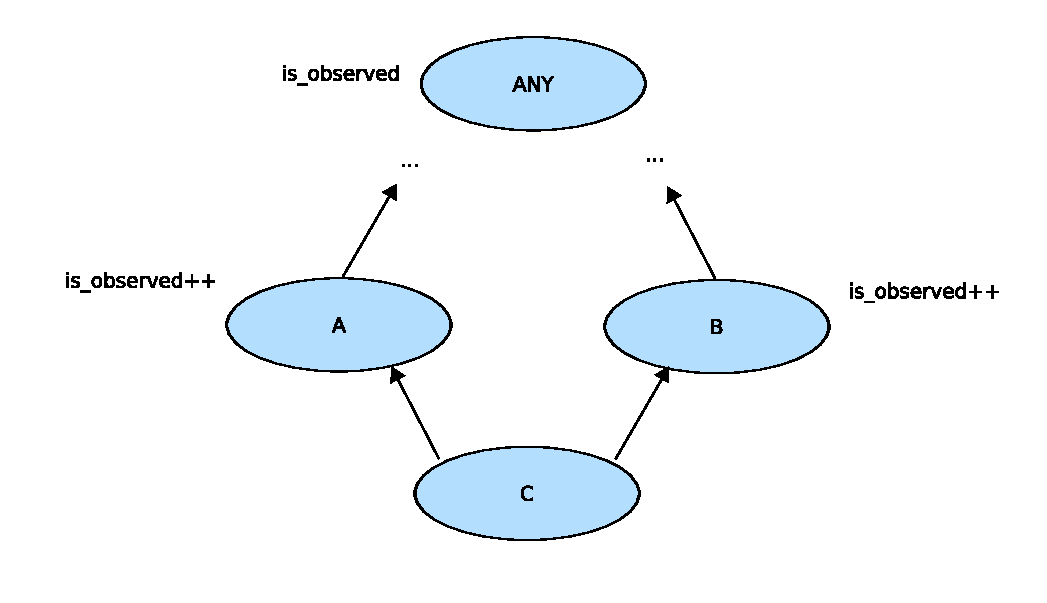
\includegraphics[width=0.9\textwidth]{illustrations/observed_query_conflicting_redefinitions}
  \caption{Example of Conflicting Redefinitions Of \feature{is\_observed}}
  \label{fig:observed_query_conflicting_redefinitions}
\end{figure}

Although this solution is more difficult to implement, it improves performance significantly, because accessing the query results in only one access to a feature instead of nested routine calls. It is possible that implementing this function as a once function can improve performance further.


\subsubsection {Implemented Solution}
Although the second solution has many advantages over the first solution, it was not chosen, because the implementation of the automatic instrumentation for it would have taken too much time. It is reasonable to replace our current implementation with this solution later, which will improve performance significantly.
%TODO evtl. noch kurz die Loesung mit UNOBSERVED_SET erklaeren.


\subsection{The Recorder}
The recorder receives the events that were passed to the program flow sink and records them to the log. To determine whether a call is an incall or outcall, it uses the \feature{is\_observed\_stack} that indicates for all routines on the call stack whether they are observed or not. Then, the recorder writes the event to the log, using the \class{CAPTURE\_SERIALIZER}.


\subsection{The Player}
The player is far more complex than the recorder, because it has to drive the application execution in contrast to the recorder which acts only as a passive sink for events (\figref{fig:implementation_player}). \\
Every time the player is invoked from the instrumentation code, it reads the next event from the \class{EVENT\_INPUT} and compares that event to the one that has just occurred. \class{EVENT\_INPUT} instantiates a different class for each event type. The events contain the same information that was written to the event log, for example the class \class{INCALL\_EVENT} has three attributes: \feature{target}, \feature{feature\_name} and \feature{arguments}, a list of entities. An \class{ENTITY} is the representation of what is written to the log for objects (\class{NON\_BASIC\hspace{0pt}\_ENTITY}) and scalar values (\class{BASIC\_ENTITY}).\\
The player uses these entities to check values received from the instrumentation code or to retrieve the corresponding values using \class{ENTITY\hspace{0pt}\_RESOLVER} in order to pass them to the application code, for example when INCALL events are replayed.\\
The deferred class \class{CALLER}, an abstraction of reflection is used to call observed routines using the routine name, the target object and the arguments. Because Eiffel lacks native reflection support, the current implementation of \class{CALLER}, \class{ERL\_CALLER} uses the reflection library generated by the Eiffel reflection library generator (Erl-G) \cite{erlg}. The reflection library adds one reflection class for each class in the universe and causes all classes of the universe and the reflection library to be part of the system, which results in vast compilation times even for small projects. To bypass this issue, it is also possible to implement an own caller specific for a project, that is able to call all observed routines; but this approach is only reasonable when the observed set is small.

\begin{figure}[ht]
  \centering
  \includegraphics[width=1\textwidth]{illustrations/implementation_player.png}
  \caption{Architecture of the player}
  \label{fig:implementation_player}
\end{figure}


\subsubsection {Resolving Entities}
\label{lbl:entity_resolving}
In the current implementation, creation procedures are instrumented in the same way as other routines, whereas the original implementation instruments creation procedures in a special way to maintain object IDs and register the objects in the reference map. To make sure that our technique can find objects to a given object ID, we use a different technique: everytime an object is passed to an unobserved routine, it is registered in the reference map. Objects only need to be resolved during replay phase, when the replay scaffolding needs to pass an observed object back to the observed set. Thus objects that never flow from the observed to the unobserved code are not interesting. During capture phase, the unobserved code must already have accessed an observed feature that returns that observed object before it can pass the object back to the observed code; or it must have created this observed object.
Therefore there is always an outgoing event, or the target of an INCALL that contains that object.

By the time of writing this report, we discovered a flaw related to this technique: because INREAD events are not captured, it is possible that unobserved code accesses an observed object without triggering an event. This could lead to the situation where unobserved code needs to pass an observed object back to observed code, without being able to resolve its object id, which would result in a failure during replay. To fix that problem it is either necessary to capture INREAD events, too or to fall back to the original implementation and register objects in their creation procedure. The original solution would result in a better performance for most applications, because objects are registered only once and not every time they're passed to the unobserved set.


\subsubsection{Replaying of Events}
Two routines of the player are invoked by the instrumentation code to notify it about a new event: \feature{put\_feature\_invocation} and \feature{put\_feature\_exit}. Using the \feature{observed\_stack}, the player then infers the type of event that has occurred. Depending on the event type, it needs to react in a different way:

\begin{description}
\item[OUTCALL] An OUTCALL event is triggered, when an unobserved routine is called from observed code. The player is invoked and compares the next event in the event log with the actual event. If the type of the event and all parameters match, it registers all retrieved objects using the \class{ENTITY\_RESOLVER} and consumes the current event. Then the player starts to simulate the unobserved routine that was called, by executing all subsequent INCALL events that are in the event log. This is necessary whenever the unobserved code called observed routines, for example when the unobserved \class{ATM\_UI} causes routine invocations on class \class{BANK} (\listref{lst:eventlog_unobserved_simulation}).  The player only executes the calls, it does not consume the associated events as this is done by the instrumentation code in the corresponding observed routines.
\begin{lstlisting}[caption=Example Event Log that Requires Simulation of the Unobserved Routine,label=lst:eventlog_unobserved_simulation]
...
OUTCALL [NON_BASIC ATM_UI 5] run
INCALL [NON_BASIC BANK 1] account_for_name [NON_BASIC STRING_8 7]
INCALLRET [NON_BASIC BANK_ACCOUNT 3]
INCALL [NON_BASIC BANK 1] deposit [NON_BASIC BANK_ACCOUNT 3] [BASIC REAL_32 "100"]
INCALLRET
...
OUTCALLRET
\end{lstlisting}
\item[OUTCALLRET] When the end of an unobserved routine that generated an OUTCALL event is reached, an OUTCALLRET event is triggered. During replay phase, this happens after the player finished the handling of the OUTCALL event. When player is then invoked again to handle the OUTCALLRET event, it reads the next event, resolves the result in the case of functions and returns to the unobserved routine.
\item[INCALL] When the instrumentation code triggers an INCALL event, the player already invoked the observed routine based on the INCALL event from the event log. Thus all the player needs to do is to consume the event and return to the observed routine.
\item[INCALLRET] The instrumentation code triggers INCALLRET events at the end of routines that caused an INCALL event. When the player receives an INCALLRET event, it compares the event to the next entry of the event log. If the events match, the player then registers the returned value and exits back to the observed routine.
\end{description}


\section{Building the Example from Source}
\sloppy % don't write path names outside the boxes...
In this section the process of building an example with capture and replay support under Linux will be described. Installing the necessary tools and setting up the modified version of Eiffel Studio, that is able to instrument applications in order to capture and replay them, will take the biggest part of this explanation.\\


\subsection{Building the Preliminaries}
The first tools we need are the  Eiffel Studio Tools \cite{estudiotools}. These will be used in many setup scripts in the examples or tests from the repository. Install these tools according to the description on the webpage.\\

The delivery of the modified Eiffel Studio was built using revision 69201 of Eiffel Studio. Building a delivery with a later version of Eiffel Studio was not tested, so it might not work. After copying the delivery to ~/estudio/Eiffel60\_gpl\_69201, it can be activated:
%TODO: @Andreas: werden die binaries von alten versionen irgendwo abgelegt? Ich glaube nicht, dass in 2 Jahren noch jemand Revision 69201 from scratch builden kann...
\bashlisting
\begin{lstlisting}
   activate_estudio 60_gpl_69201
\end{lstlisting}

Since the Eiffel compiler is available, Gobo \cite{gobo} can be downloaded from svn and then bootstrapped (Revision 6001 was successfully tested).
\begin{lstlisting}
svn co -r6001 https://gobo-eiffel.svn.sourceforge.net/svnroot/gobo-eiffel/gobo/trunk ~/capture_replay/gobo
export GOBO=~/capture\_replay/gobo
export PATH=$GOBO/bin:$PATH
$GOBO/work/bootstrap/bootstrap.sh gcc ise
\end{lstlisting}

It is assumed that all commands in the following steps are executed in the same session to keep the environment variables.\\
As all preliminaries are installed, Erl-G \cite{erlg} can be downloaded and built. Revision 719 of Erl-G was tested together with selective capture and replay for Eiffel.
\begin{lstlisting}
svn co -r719 https://svn.origo.ethz.ch/autotest/trunk/erl_g ~/capture_replay/erl_g
export ERL_G=~/capture_replay/erl_g
export PATH=$ERL_G/bin:$PATH
cd $ERL_G
export ISE_LIBRARY=$EIFFEL_SRC
geant install
geant compile
\title{Selective Capture and Replay for Eiffel
\end{lstlisting}

To build a delivery of the modified Eiffel Studio, execute these commands: (this will take a few hours).
\begin{lstlisting}
cd ~/capture_replay/
mkdir es
svn co https://eiffelsoftware.origo.ethz.ch/svn/es/branches/capture_replay es
export EIFFEL_SRC=~/capture_replay/es/Src
cd es
geant -b $EIFFEL_SRC/scripts/build.eant build_es
\end{lstlisting}

Before an example can be built, the delivery that was just created needs to be set as default instance of Eiffel Studio
\begin{lstlisting}
cd ~/estudio
ln -s ~/capture_replay/es/EiffelXX EiffelCR
activate_estudio CR
\end{lstlisting}

In order to make the created Eiffel Studio use a modified version of the runtime, it is necessary to recompile the runtime with modified CFLAGS. The new version of the runtime then needs to be installed in the delivery.

It is not possible to directly build Eiffel Studio with the modified version of the runtime, because the changes in the runtime are not compatible to Eiffel's store mechanism. This would render Eiffel Studio unusable, because it relies on this mechanism during the build process.
\begin{lstlisting}
export CFLAGS='-DCAPTURE_REPLAY' 
cd $EIFFEL_SRC
#build the runtime from scratch (clobber the old one)
geant -b scripts/build.eant compile_runtime
cd $ISE_EIFFEL/studio/spec/linux-x86/lib
rm *
cp $EIFFEL_SRC/C/run-time/lib* .
\end{lstlisting}


\subsection{Building an Example}
Now, all necessary tools are installed, the corresponding environment variables set and we can start to build an example.\\
First we need to add reflection support to the example project. Erl G will generate reflection classes for us. If the environment variables are correctly set, the geant script invokes Erl G automatically. \\
At the moment Erl-G does not support overrides because this feature is missing in the Gobo parser. Therefore it is necessary to override the necessary classes manually. There are two geant tasks that take care of this:

\begin{itemize}
\item \identifier{patch\_elks} makes the manual override by copying the modified elks classes from \$EIFFEL\_SRC/library/base/capture\_replay/elks\_overrides to \$ISE\_LIBRARY/library/base/elks \\
\item \identifier{unpatch\_elks} restores the original state by copying the original elks classes from \$EIFFEL\_SRC/library/base/elks to \$ISE\_LIBRARY/library/base/elks .
\end{itemize}

\begin{lstlisting}
cd ~/capture_replay/es/examples/capture_replay/command_line
geant install
\end{lstlisting}

The example can now be opened with the modified version of Eiffel Studio. Make sure that the CFLAGS are still set to '-DCAPTURE\_REPLAY'. Otherwise it will not be possible to build the example.

An environment variable is used to control capture and replay of the instrumented application. Whether the application is captured or replayed depends on the value of the environment variable \identifier{CR\_MODE} at the application startup. The following values are supported:

\begin{description}
 \item [not set] When \identifier{CR\_MODE} is not set, selective capture and replay will be disabled.
 \item [\identifier{capture}] When the mode is set to \identifier{capture}, the program execution will be captured.
 \item [\identifier{replay}] When \identifier{CR\_MODE} is set to \identifier{replay}, the program will be replayed.
 \item [\identifier{log\_replay}] This mode replays the program and writes an event log in parallel. This event log has the same structure as the one that is written during capture phase. If the replay runs correct, the two logs are identical, therefore this feature can be used for testing.
\end{description}

Setting the environment variable controls the initialization of \identifier{program\_flow\_sink}. To set up all other necessary parameters for capture and replay phase, the creation procedure of the root class is used. This setup code needs to be inserted into applications that are to be captured and replayed. The setup code of the example can be used as a reference.

\fussy